\documentclass[12pt, atypical, journal]{article}

\usepackage[utf8]{inputenc}
\usepackage[spanish,es-tabla]{babel}
\usepackage{geometry}
\geometry{letterpaper, margin=2.54cm}
\usepackage{times}
\usepackage{setspace}
\onehalfspacing
\usepackage{graphicx}
\usepackage{booktabs}
\usepackage{longtable}
\usepackage{titlesec}
\usepackage{hyperref}
\usepackage{caption}

\newenvironment{hangparas}[2]{\setlength{\parindent}{-#1}\setlength{\leftmargin}{#1}\everypar{\hangindent=#1}}{\par}

\hypersetup{
   colorlinks=true,
   linkcolor=black,
   filecolor=black,     
   urlcolor=blue,
   citecolor=black
}

\titleformat{\section}{\normalfont\Large\bfseries}{\thesection.}{0.5em}{}
\titleformat{\subsection}{\normalfont\large\bfseries}{\thesubsection.}{0.5em}{}
\titleformat{\subsubsection}{\normalfont\normalsize\bfseries\itshape}{\thesubsubsection.}{0.5em}{}

\usepackage{pgffor}
\usepackage{longtable}
\usepackage{pdfpages}
\usepackage{float}
\usepackage{listings}
\usepackage{xcolor}
\lstset{
    basicstyle=\ttfamily\footnotesize,
    breaklines=true,
    frame=single,
    showstringspaces=false,
    tabsize=2,
    extendedchars=true,
    literate={á}{{\'a}}1 {é}{{\'e}}1 {í}{{\'i}}1 {ó}{{\'o}}1 {ú}{{\'u}}1 {Á}{{\'A}}1 {É}{{\'E}}1 {Í}{{\'I}}1 {Ó}{{\'O}}1 {Ú}{{\'U}}1 {ñ}{{\~n}}1 {Ñ}{{\~N}}1
}

\begin{document}

% ==============================================================================
% 1. PORTADA
% ==============================================================================
\begin{titlepage}
   \begin{center}
       \vspace*{1cm}
      
       {\Large\bfseries UNIVERSIDAD POLITÉCNICA DE CHIAPAS} \\[0.5cm]
       {\large\bfseries INGENIERÍA EN TECNOLOGÍAS DE LA INFORMACIÓN E INNOVACIÓN DIGITAL} \\[1.5cm]
      
       \vfill
      
       {\Large\bfseries REPORTE DE PROYECTO INTEGRADOR II} \\[1cm]
      
       \textbf{Nombre del Proyecto:} \\
       {\large LecturaMétrica: Plataforma Web para la Gestión Automatizada, Analítica y Gamificada del Hábito Lector} \\[1.5cm]
      
       \vfill
      
       \textbf{Integrantes del Equipo:} \\[0.3cm]
       {\large Patricia Alejandra Clemente Chacón (Matrícula: 251237)} \\
       {\large Nínive Argelia Pérez González (Matrícula: 251239)} \\
       {\large Mónica Jamileth Velázquez García (Matrícula: 243729)} \\[1.5cm]
      
       \textbf{Docente:} \\
       {\large Ballinas Garcia Sirgei} \\[1.5cm]
       
       \textbf{Grado y Grupo:} \\
       {\large 5 B} \\[1.5cm]
      
       \vfill
      
       \textbf{Fecha de entrega:} \\
       {\large 13 de junio de 2026}
      
       \vspace*{1cm}
   \end{center}
\end{titlepage}

\newpage

% ==============================================================================
% ÍNDICES
% ==============================================================================
\tableofcontents
\newpage

% ==============================================================================
% 2. Introducción
% ==============================================================================
\section{Introducción}

\subsection{Antecedentes y evidencia}
Las herramientas existentes en el mercado presentan un vacío operativo significativo. Por una parte, existen redes sociales abiertas orientadas a la publicación de textos (como Wattpad o Webtoon) que no ofrecen herramientas métricas personales; por otra parte, plataformas de catálogo literario (como Goodreads) o plantillas de hojas de cálculo (Excel) dependen de un llenado manual repetitivo. Experiencias y estudios de usabilidad en aplicaciones de registro de hábitos demuestran que la alta fricción operativa —es decir, la pérdida de tiempo y el esfuerzo cognitivo que implica registrar datos a mano— es la causa primordial por la cual los usuarios abandonan el uso de estas herramientas durante las primeras semanas, generando frustración e interrumpiendo su ciclo de lectura.

\subsection{Descripción del problema en su contexto}
En la actualidad, muchas personas que desean desarrollar o mantener el hábito de la lectura se enfrentan a la falta de herramientas accesibles para cuantificar su rendimiento diario. En el contexto cotidiano, los lectores se dividen en dos grupos principales que experimentan dificultades similares: por un lado, los lectores principiantes sufren de desmotivación y abandono prematuro al sentir que leer es una actividad aislada y difícil de medir; por otro lado, los lectores habituales —que consumen libros, mangas o novelas gráficas— carecen de un espacio centralizado para organizar grandes volúmenes de capítulos. Al depender de bitácoras manuales o notas dispersas, el control del avance se vuelve una tarea tediosa que termina por interrumpir la constancia del usuario.

\subsection{Objetivo General}
Desarrollar una plataforma web llamada LecturaMétrica que permita optimizar el hábito lector en el público general mediante herramientas de seguimiento automatizado, análisis estadístico multiformato y gestión personalizada de bibliotecas digitales, utilizando un ecosistema tecnológico compuesto por Next.js, Java con Spring Boot y PostgreSQL bajo un modelo de desarrollo híbrido.

\subsection{Objetivos Específicos}
\begin{enumerate}
   \item Diseñar e implementar el módulo de biblioteca personal mediante operaciones CRUD de obras, optimizándolo a través de una arquitectura híbrida de ingesta de datos que combine el consumo de APIs externas de metadatos y rastreadores web para automatizar la extracción de portadas, capítulos y géneros, eliminando la fricción del registro manual.
   \item Desarrollar un componente interactivo de cuantificación de progreso en el \textit{front-end} que ofrezca un flujo dual de captura: un temporizador en tiempo real para la medición automatizada de sesiones activas, y un formulario de registro manual retroactivo para asegurar la flexibilidad de recolección de datos sin importar el entorno del usuario.
   \item Programar la lógica algorítmica para la gestión de un motor de gamificación que procese el cálculo automatizado de rachas consecutivas de días leyendo (\textit{streaks}), récords históricos, asignación de insignias y la inyección automatizada de un ``Radar de Curiosidades'' basado en las preferencias del usuario.
   \item Construir el sistema de mensajería asíncrona ``Buzón del Lector'', implementando las reglas de negocio y filtros necesarios en el servidor para la distribución aleatoria y anónima de micro-reseñas en ciclos controlados de bloqueo y apertura de 24 horas.
   \item Estructurar un \textit{dashboard} analítico dinámico utilizando componentes gráficos interactivos en Next.js para representar la distribución de lectura por géneros literarios, promedios de velocidad lectora real, estimaciones predictivas de finalización de obras y líneas de tiempo de metas cumplidas.
   \item Evaluar el impacto y usabilidad de la plataforma mediante la recolección de datos cuantitativos en una muestra de un mínimo de 40 usuarios reales durante un periodo de 20 días naturales, validando estadísticamente el incremento del tiempo promedio de lectura diario y la tasa de retención activa.
\end{enumerate}

\subsection{Justificación del desarrollo del proyecto}
El desarrollo de \textbf{LecturaMétrica} es fundamental porque ofrece una herramienta que elimina la carga operativa del lector moderno mediante la automatización de datos a través del consumo de servicios externos (como la API de Open Library). Socialmente, aporta una propuesta innovadora para mitigar el aislamiento del lector sin exponerlo a la saturación o toxicidad de las redes sociales tradicionales, lográndolo mediante un intercambio anónimo y controlado de cartas literarias cada 24 horas. Académicamente, el proyecto permite aplicar conceptos avanzados de ingeniería de software, arquitectura web e integración de bases de datos, permitiendo además una evaluación cuantitativa real para medir el incremento del tiempo diario de lectura en un grupo de prueba.


\subsection{Alcances y limitaciones}
El alcance del proyecto contempla el desarrollo de funcionalidades básicas para la gestión de cuentas de usuario, una biblioteca personal para catalogar obras, un temporizador para cronometrar las sesiones de lectura, un tablero de estadísticas y un buzón para intercambiar recomendaciones literarias entre usuarios. Como limitaciones, el sistema no almacena ni visualiza archivos de libros digitales (como PDF o EPUB) por cuestiones de derechos de autor, ni incluye salas de chat públicas en tiempo real.

\subsection{Entregables esperados}

\subsection{Actividades}

\subsection*{Cronograma de actividades}
\addcontentsline{toc}{subsection}{Diagrama de Grantt}
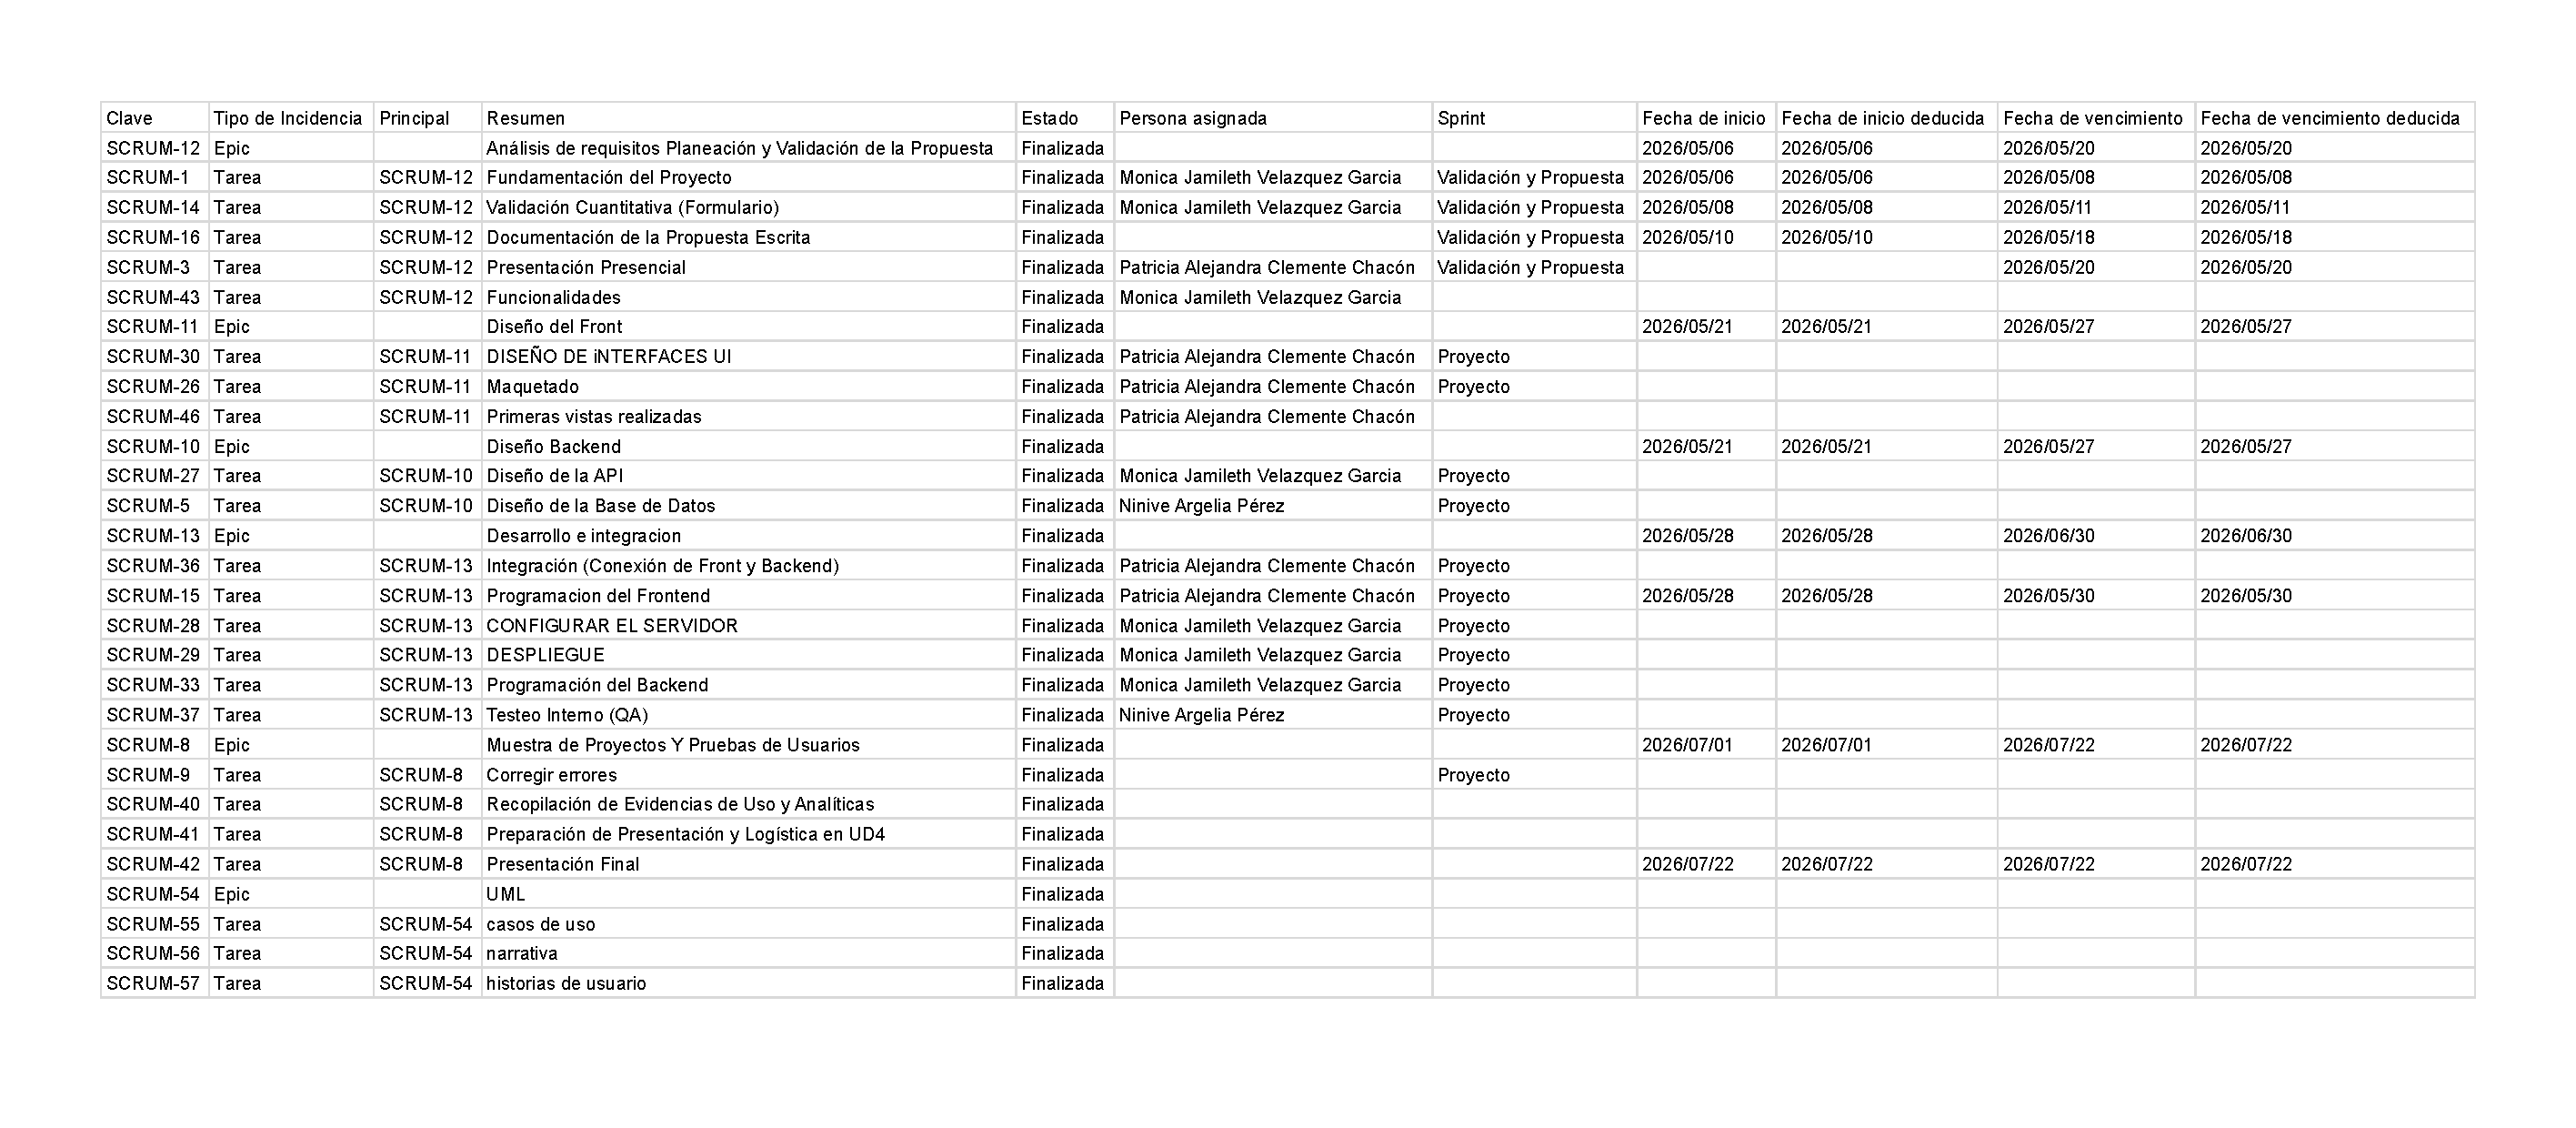
\includepdf[pages=-]{./anexos/DiagramaGrant.pdf}

% ==============================================================================
% 2. MARCO REFERENCIAL
% ==============================================================================
\section{Marco Referencial}

\subsection{Marco teórico}
El desarrollo de sistemas de gestión de hábitos de lectura y seguimiento analítico se sustenta en diversos conceptos teóricos y metodológicos provenientes de la ingeniería de software, la psicología conductual y el diseño de sistemas de información. En primer lugar, la arquitectura desacoplada y la Arquitectura Limpia (\textit{Clean Architecture}) propuesta por Robert C. Martin \cite{martin2018} establecen un marco estricto para separar las reglas de negocio de los detalles de infraestructura, frameworks y interfaces de usuario, lo cual garantiza la mantenibilidad y escalabilidad a largo plazo de aplicaciones complejas.

Asimismo, en el ámbito de la psicología cognitiva y la formación de hábitos, las teorías de modificación de conducta sugieren que la reducción de la fricción operativa y la integración de estímulos visuales incrementan significativamente la constancia de los usuarios. En este contexto, la gamificación asíncrona actúa como un mecanismo que, mediante recompensas intermitentes, rachas de lectura (\textit{streaks}) y sistemas de progresión, disminuye la resistencia cognitiva y fomenta la motivación intrínseca sin saturar al usuario con dinámicas sociales invasivas.

\subsection{Estado de la tecnología}

\begin{enumerate}
    \item \textbf{Gestores masivos de bibliotecas (Goodreads, StoryGraph):} Plataformas enfocadas en la catalogación exhaustiva y la reseña literaria. Aunque cuentan con bases de datos inmensas, carecen de herramientas de seguimiento en tiempo real (como temporizadores en web). Además, su principal base de usuarios y diseño nativo se centra en el idioma inglés.
    \item \textbf{Medidores de hábitos y sesiones (Bookmory, Bookly):} Son las herramientas funcionalmente más cercanas al propósito de este proyecto, ya que integran temporizadores, calendarios y estadísticas detalladas. Sin embargo, su enfoque es estrictamente individualista y cerrado, aislando al lector. Aplicaciones como Bookly suelen bloquear funciones hasta pagar una suscripción, mientras que Bookmory carece de mecánicas de interacción comunitaria.
    \item \textbf{Plataformas de autoedición y consumo serializado (Wattpad, Webtoon, Lilithum):} Su núcleo no es la medición del hábito, sino la publicación y el consumo de contenido original. Su componente social es síncrono, directo y a menudo invasivo (comentarios por párrafo o capítulo), lo cual no fomenta la disciplina lectora de obras externas, sino la permanencia dentro de su propio ecosistema de contenido.
\end{enumerate}

A pesar de la popularidad de estas herramientas, el usuario hispanohablante se enfrenta a barreras de idioma o a la falta de una plataforma que equilibre el seguimiento cuantitativo con una motivación comunitaria sana.

\begin{table}[htpb]
\centering
\caption{Análisis comparativo de plataformas de gestión y fomento de lectura}
\label{tab:comparativa_apps}
\resizebox{\textwidth}{!}{
\begin{tabular}{@{}lcccccc@{}}
\toprule
\textbf{Plataforma} & \textbf{Registro por API} & \textbf{Temporizador} & \textbf{Analíticas} & \textbf{Gamificación} & \textbf{Interacción Social} & \textbf{Idioma Nativo} \\
\midrule
\textbf{Goodreads} & Manual / ISBN & No & Básicas & Reto Anual & Foros abiertos & Inglés \\
\textbf{StoryGraph} & Manual / ISBN & No & Avanzadas & Reto Anual & Seguidores & Inglés \\
\textbf{Bookly} & Manual / ISBN & Sí & Avanzadas & Insignias & Nula & Inglés \\
\textbf{Bookmory} & Manual / ISBN & Sí & Avanzadas & Rachas / Calendario & Nula & Multi (Traducido) \\
\textbf{Wattpad / Webtoon / Lilithum} & N/A (Interno) & No & N/A & N/A & Comentarios directos & Español / Multi \\
\midrule
\textbf{LecturaMétrica (Propuesta)} & \textbf{Sí} & \textbf{Sí} & \textbf{Avanzadas} & \textbf{Rachas / Insignias} & \textbf{Buzón Asíncrono} & \textbf{Español} \\
\bottomrule
\end{tabular}
}
\end{table}

Como se observa en la comparativa, \textbf{LecturaMétrica} se posiciona como una solución superior en su nicho al tomar las mejores mecánicas de medición (presentes en aplicaciones como Bookmory) y potenciarlas mediante la inyección de un componente social controlado. El modelo del ``Buzón del Lector'' introduce un intercambio asíncrono y anónimo que genera expectativa y curiosidad sin la presión de las redes sociales tradicionales. Sumado a su arquitectura de ingesta automatizada y su diseño nativo en español, la plataforma elimina la resistencia cognitiva, garantizando una mayor retención del usuario.


\subsection{Contexto tecnológico}
\begin{itemize}
   \item \textbf{Next.js, React y Tailwind CSS:} Framework de desarrollo \textit{front-end} basado en JavaScript y biblioteca de estilos que permite la renderización eficiente de interfaces de usuario basadas en componentes. Su gestión nativa de estados dinámicos combinada con un diseño ágil y adaptable facilita la construcción de gráficos estadísticos interactivos y tableros analíticos en tiempo real.
   \item \textbf{Java y Spring Boot:} Lenguaje de programación fuertemente tipado acoplado a un framework robusto para el desarrollo del \textit{back-end}. Su motor de inversión de control (IoC) e inyección de dependencias permite aislar rígidamente las reglas de negocio del motor de gamificación y la seguridad del servidor.
   \item \textbf{Spring Data JPA e Hibernate:} Tecnologías de mapeo objeto-relacional (ORM) que abstraen la capa de datos en Java, transformando las entidades de software en tablas de bases de datos relacionales y automatizando las consultas transaccionales de alta velocidad.
   \item \textbf{PostgreSQL:} Sistema de gestión de bases de datos relacionales (RDBMS) de código abierto, seleccionado por su alta integridad cuantitativa, soporte avanzado para tipos de datos complejos y eficiencia en el almacenamiento seguro de variables métricas acumuladas.
\end{itemize}

\newpage

% ==============================================================================
% 3. METODOLOGÍA Y DESARROLLO DEL PROYECTO
% ==============================================================================
\section{Metodología y desarrollo del proyecto}

\subsection{Levantamiento de requerimientos}
El levantamiento de requerimientos para el sistema \textbf{LecturaMétrica} se llevó a cabo mediante la aplicación de técnicas de investigación de campo y análisis documental. Se realizaron entrevistas y cuestionarios preliminares dirigidos a usuarios lectores para identificar las fricciones operativas comunes en el control manual de lecturas, tales como el abandono de bitácoras en papel y la dispersión de información. Asimismo, se examinaron flujos de trabajo de plataformas existentes para determinar las necesidades esenciales que el sistema debía automatizar.

\subsection{Análisis de requerimientos}
A partir de la información recopilada, se procedió al análisis y estructuración de los requerimientos del sistema en dos categorías principales:
\begin{itemize}
    \item \textbf{Requerimientos Funcionales:} Se definieron las capacidades operativas esenciales que la plataforma debe garantizar, tales como el registro e inicio de sesión seguro de usuarios, la gestión del catálogo literario multiformato (libros, mangas, webtoons), la asociación automática de metadatos mediante servicios externos, la actualización incremental de sesiones de lectura y el cálculo automatizado de métricas y rachas de lectura (\textit{streaks}).
    \item \textbf{Requerimientos No Funcionales:} Se establecieron los estándares de calidad, seguridad y rendimiento. Esto incluye cifrado seguro de credenciales mediante BCrypt, protección de rutas y endpoints mediante tokens JWT, alta disponibilidad del servicio y adaptabilidad responsiva de la interfaz de usuario en diversos dispositivos.
\end{itemize}

\subsection{Diseño}
El diseño de la solución se estructuró bajo un modelo de arquitectura desacoplada cliente-servidor y un enfoque centrado en el usuario, integrando los siguientes componentes:
\begin{itemize}
    \item \textbf{Arquitectura y Patrones de Diseño:} Implementación de \textit{Clean Architecture} en el servidor para separar de forma estricta las reglas de negocio, la capa de aplicación y la infraestructura.
    \item \textbf{Historias de Usuario y Modelado Funcional:} Definición de épicas e historias de usuario organizadas por módulos (gestión de biblioteca, sesiones de lectura, perfil, seguridad y buzón asíncrono) para estructurar los requerimientos desde la perspectiva del lector y del administrador.
    \item \textbf{Narrativas de Casos de Uso:} Especificación formal de las interacciones entre los actores y el sistema, documentando flujos normales y alternativos para operaciones críticas como el registro de sesiones de lectura.
    \item \textbf{Prototipos de Interfaces y Maquetado (Figma):} Diseño previo de las pantallas, flujos de navegación y componentes visuales mediante wireframes y prototipos interactivos en Figma, garantizando una experiencia de usuario intuitiva y coherente antes de su codificación.
    \item \textbf{Diagramas del Sistema:} Modelado mediante diagramas de casos de uso UML para delimitar los roles del lector y del administrador, junto con el diagrama Entidad-Relación preliminar y definitivo.
    \item \textbf{Base de Datos Relacional:} Diseño de un esquema normalizado en PostgreSQL compuesto por 22 tablas organizadas en cinco dominios de negocio (usuarios, catálogo, biblioteca personal, gamificación y buzón asíncrono), incorporando estrategias híbridas de identificadores UUID y BIGINT, así como control de borrado suave (\textit{soft delete}).
    \item \textbf{Interfaces Modulares:} Construcción visual basada en componentes reactivos con Next.js y Tailwind CSS, separando la aplicación web progresiva (PWA) del usuario y el panel de control administrativo (\textit{Dashboard}).
\end{itemize}

\subsection{Implementación}
La implementación del sistema se ejecutó de forma modular y descentralizada en tres repositorios independientes para asegurar un bajo acoplamiento:
\begin{itemize}
    \item \textbf{Desarrollo del Backend:} Construido en Java 21 utilizando Spring Boot, Spring Data JPA e Hibernate. Se programaron los controladores REST, servicios de negocio, validaciones de seguridad con JWT, el consumo de la API externa de Open Library para la ingesta automatizada de portadas y metadatos, y los algoritmos de cálculo de rachas e insignias.
    \item \textbf{Desarrollo del Frontend (PWA y Admin):} Codificado en Next.js con TypeScript y Tailwind CSS, implementando el enrutamiento por App Router, la gestión de estados globales y componentes optimizados para la visualización de estadísticas, temporizadores de lectura en tiempo real y el buzón de recomendaciones anónimas.
    \item \textbf{Control de Versiones y Despliegue:} Gestión del código fuente mediante Git y GitHub, apoyándose en contenedores Docker y servicios en la nube para la persistencia transaccional y el alojamiento de recursos multimedia en Cloudinary.
\end{itemize}

\subsection{Pruebas}
Esta sección documenta el proceso de aseguramiento de calidad de software (QA) aplicado al proyecto, incluyendo el entorno de pruebas, las categorías evaluadas, los resultados obtenidos y los defectos identificados.

\subsubsection{Calidad de software (QA)}

\paragraph{Objetivo del testing}
[Describir el propósito y alcance general de la estrategia de pruebas, especificando qué flujos o componentes clave se validaron antes del paso a producción.]

\paragraph{Entorno de pruebas}
\begin{table}[H]
\centering
\small
\begin{tabular}{|l|p{9cm}|}
\hline
\textbf{Aspecto} & \textbf{Detalle} \\ \hline
Aplicación evaluada & [Especificar plataformas o aplicaciones evaluadas] \\ \hline
Versión de la app & [Indicar versión y build] \\ \hline
Versión web & [Indicar commit, rama o release web] \\ \hline
URL de staging & \url{[Insertar URL de prueba o staging]} \\ \hline
Ambiente de backend & [Describir ambiente de backend y datos de prueba utilizados] \\ \hline
Herramientas de gestión & [Indicar herramientas para gestión de bugs, casos de prueba y dispositivos] \\ \hline
Periodo de ejecución & [Fecha de inicio al Fecha de fin] \\ \hline
\end{tabular}
\caption{Entorno y parámetros generales de pruebas.}
\label{tab:qa_entorno}
\end{table}

\paragraph{Dispositivos y navegadores utilizados}
\begin{table}[H]
\centering
\small
\begin{tabular}{|l|l|p{6cm}|}
\hline
\textbf{Categoría} & \textbf{Dispositivos / Navegadores} & \textbf{Versión de SO / Motor} \\ \hline
Móvil - iOS & [Lista de dispositivos iOS] & [Versiones de iOS] \\ \hline
Móvil - Android & [Lista de dispositivos Android] & [Versiones de Android] \\ \hline
Navegador - Desktop & [Navegadores de escritorio] & [Versiones o estándar] \\ \hline
Navegador - Mobile Web & [Navegadores móviles] & [Motores utilizados] \\ \hline
Resoluciones web & [Resoluciones evaluadas] & --- \\ \hline
\end{tabular}
\caption{Matriz de dispositivos y navegadores.}
\label{tab:qa_dispositivos}
\end{table}

\paragraph{Categorías de prueba ejecutadas}
\begin{enumerate}
    \item \textbf{Pruebas funcionales:}
    \begin{itemize}
        \item Flujos de usuario end-to-end: registro, login, recuperación de contraseña y flujo principal del negocio.
        \item Casos de borde ante datos inválidos, campos vacíos, caracteres especiales y valores extremos.
        \item Sincronización de datos entre la interfaz web y la aplicación móvil.
        \item Validaciones de formularios y mensajes de error.
    \end{itemize}
    \item \textbf{Pruebas de interfaz y experiencia de usuario (UI/UX):}
    \begin{itemize}
        \item Responsividad web en laptops, tablets y monitores ultra-wide.
        \item Consistencia de diseño (colores, tipografías, iconografía) en las plataformas.
        \item Accesibilidad (contraste, tamaño de fuente y navegación).
    \end{itemize}
    \item \textbf{Pruebas de rendimiento:}
    \begin{itemize}
        \item Tiempos de carga inicial y respuesta del sitio web.
        \item Comportamiento de red ante conexiones lentas o pérdida de conexión.
        \item Pruebas de carga y estrés en backend ante usuarios concurrentes.
    \end{itemize}
    \item \textbf{Pruebas de compatibilidad y portabilidad:}
    \begin{itemize}
        \item Verificación cross-browser (Chromium, WebKit, Gecko).
        \item Adaptabilidad a distintos tamaños de pantalla y orientación.
    \end{itemize}
    \item \textbf{Pruebas de seguridad básicas:}
    \begin{itemize}
        \item Manejo de sesiones, expiración correcta y bloqueo de rutas protegidas.
        \item Almacenamiento local seguro de tokens y contraseñas cifradas.
        \item Comunicación segura mediante HTTPS/TLS y control de acceso.
    \end{itemize}
    \item \textbf{Pruebas de integración (API / terceros):}
    \begin{itemize}
        \item Integraciones externas y manejo de errores de API ante códigos 4xx/5xx.
    \end{itemize}
    \item \textbf{Pruebas de localización e idioma:}
    \begin{itemize}
        \item Verificación de formatos de fecha, textos y que las traducciones no rompan el diseño.
    \end{itemize}
\end{enumerate}

\paragraph{Aspectos técnicos por capa}
Además de las categorías generales, se evaluaron aspectos técnicos propios de cada capa:

\begin{itemize}
    \item \textbf{Frontend — Aplicación web}
    \begin{itemize}
    \item \textit{Rendimiento (Core Web Vitals):} Se evaluaron los indicadores de rendimiento web bajo los estándares recomendados por Google para garantizar una experiencia fluida en la interfaz de usuario de la plataforma:
    \begin{table}[H]
    \centering
    \small
    \begin{tabular}{|l|p{5cm}|p{4.5cm}|}
    \hline
    \textbf{Métrica} & \textbf{Qué mide} & \textbf{Umbral recomendado} \\ \hline
    LCP (Largest Contentful Paint) & Tiempo en renderizar el contenido principal & Menor a 2.5 segundos \\ \hline
    INP (Interaction to Next Paint) & Tiempo de respuesta ante clic o escritura & Menor a 200 ms \\ \hline
    CLS (Cumulative Layout Shift) & Estabilidad visual durante la carga & Menor a 0.1 \\ \hline
    \end{tabular}
    \caption{Métricas Core Web Vitals.}
    \label{tab:core_web_vitals}
    \end{table}
    \item Gestión de estado, almacenamiento local y persistencia de datos ante recarga.
    \item Consumo de APIs y manejo de errores HTTP ante timeouts.
\end{itemize}

\begin{table}[h!]
    \centering
    \caption{Resultados de Auditoría Lighthouse para Lectura Métrica}
    \begin{tabular}{|l|c|}
        \hline
        \textbf{Métrica / Categoría} & \textbf{Puntuación / Valor} \\ \hline
        Rendimiento (Performance) & 100 / 100 \\ \hline
        Accesibilidad (Accessibility) & 86 / 100 \\ \hline
        Buenas Prácticas (Best Practices) & 100 / 100 \\ \hline
        SEO & 100 / 100 \\ \hline
        First Contentful Paint (FCP) & 0.4 s \\ \hline
        Largest Contentful Paint (LCP) & 0.6 s \\ \hline
        Speed Index & 0.8 s \\ \hline
        Total Blocking Time (TBT) & 60 ms \\ \hline
        Cumulative Layout Shift (CLS) & 0 \\ \hline
        Time to Interactive (TTI) & 0.6 s \\ \hline
    \end{tabular}
    \label{tab:lighthouse-metrics}
\end{table}
    \item \textbf{Backend / API — Integración entre plataformas}
    \begin{itemize}
        \item Concurrencia y sincronización en tiempo real.
        \item Consistencia de reglas de negocio y validación de campos idénticos entre clientes.
    \end{itemize}
\end{itemize}

\paragraph{Métricas y resultados (estado de salud)}
\begin{table}[H]
\centering
\small
\begin{tabular}{|l|c|c|p{4.5cm}|}
\hline
\textbf{Estado de los casos de prueba} & \textbf{Cantidad} & \textbf{Porcentaje} & \textbf{Observaciones} \\ \hline
Exitosos (Passed) & [Cantidad] & [\%] & [Observación] \\ \hline
Fallidos (Failed) & [Cantidad] & [\%] & [Observación] \\ \hline
Bloqueados (Blocked) & [Cantidad] & [\%] & [Observación] \\ \hline
\textbf{Total ejecutados} & \textbf{[Total]} & \textbf{100\%} & \\ \hline
\end{tabular}
\caption{Resumen de ejecución de casos de prueba.}
\label{tab:qa_resultados}
\end{table}

[Redactar un breve análisis interpretando la tasa de éxito obtenida y los riesgos detectados.]



\paragraph{Reporte de defectos (bug log)}
Criterios de clasificación:
\begin{itemize}
    \item \textbf{Bloqueante / crítico:} La app se cierra inesperadamente, no permite iniciar sesión o impide flujos esenciales.
    \item \textbf{Mayor:} Una funcionalidad importante falla, pero existe una alternativa (workaround).
    \item \textbf{Menor / cosmético:} Errores tipográficos, botones desalineados o detalles visuales menores.
\end{itemize}

Defectos encontrados:
\begin{table}[H]
\centering
\small
\begin{tabular}{|l|l|p{5cm}|l|l|}
\hline
\textbf{ID} & \textbf{Severidad} & \textbf{Descripción} & \textbf{Módulo / Plataforma} & \textbf{Estado} \\ \hline
BUG-001 & [Severidad] & [Descripción del defecto] & [Módulo / Plataforma] & [Estado] \\ \hline
BUG-002 & [Severidad] & [Descripción del defecto] & [Módulo / Plataforma] & [Estado] \\ \hline
\end{tabular}
\caption{Registro de defectos encontrados (Bug Log).}
\label{tab:bug_log}
\end{table}

Distribución por severidad:
\begin{table}[H]
\centering
\small
\begin{tabular}{|l|c|c|p{5.5cm}|}
\hline
\textbf{Nivel de severidad} & \textbf{Cantidad} & \textbf{\% del total} & \textbf{Criterio de salida} \\ \hline
Crítico / Blocker & [Cant] & [\%] & [Criterio] \\ \hline
Mayor & [Cant] & [\%] & [Criterio] \\ \hline
Menor / Cosmético & [Cant] & [\%] & [Criterio] \\ \hline
\end{tabular}
\caption{Distribución de defectos por severidad.}
\label{tab:defectos_severidad}
\end{table}

\paragraph{Conclusión de QA y estado del release}
[Describir las conclusiones generales de la fase de pruebas, la solidez funcional encontrada y el impacto de los defectos identificados.]

\paragraph{Recomendaciones de QA:}
\begin{itemize}
    \item Incluir recomendaciones de acción basadas en los resultados.
\end{itemize}

\noindent\textbf{Veredicto QA:} \textbf{[APTO / NO APTO]} para producción en su estado actual — [condicionado o justificación del veredicto].

\section{Implementación}

\subsection{Repositorios del proyecto y control de versiones}
El desarrollo del ecosistema \textbf{LecturaMétrica} se gestionó mediante el control de versiones distribuido Git y la plataforma de alojamiento GitHub. 

Para garantizar un bajo acoplamiento arquitectónico, mantener prácticas de Arquitectura Limpia y facilitar el ciclo de despliegue independiente de cada interfaz, el código fuente se encuentra versionado en tres repositorios oficiales:

\begin{table}[H]
\centering
\footnotesize
\begin{tabular}{|p{3.8cm}|p{6.2cm}|p{4.5cm}|}
\hline
\textbf{Módulo del Ecosistema} & \textbf{Responsabilidad y Tecnología} & \textbf{Enlace al Repositorio (GitHub)} \\ \hline
\textbf{Backend (API RESTful)} & Núcleo lógico del sistema, validación de reglas de negocio, cálculo de rachas y conexión a PostgreSQL. Desarrollado en Java y Spring Boot. & \url{https://github.com/SoftFairies/Backend.git} \\ \hline
\textbf{Frontend 1: Usuario (PWA)} & Aplicación Web Progresiva para lectores finales con cronómetro de lectura asíncrono y catálogo personal. Desarrollada en Next.js. & \url{https://github.com/SoftFairies/LecturaMetrica-Usuario.git} \\ \hline
\textbf{Frontend 2: Dashboard Admin} & Interfaz web cerrada (back-office) para la gestión de usuarios, monitoreo del sistema y administración de catálogo. Desarrollada en Next.js. & \url{https://github.com/SoftFairies/LecturaMetrica-Admin.git} \\ \hline
\end{tabular}
\caption{Repositorios oficiales y código fuente del sistema LecturaMétrica.}
\label{tab:repositorios_github}
\end{table}

\vspace{0.2cm}

\subsection{Despliegue}
El proceso de despliegue a producción del sistema \textbf{LecturaMétrica} se concibe bajo una estrategia automatizada y desacoplada para garantizar la estabilidad operativa del entorno real:
\begin{itemize}
    \item \textbf{Despliegue del Backend:} Tras superar las fases de pruebas unitarias e integración, el núcleo de servicios desarrollado en Spring Boot se empaqueta mediante contenedores Docker, configurando las variables de entorno definitivas de conexión a la base de datos PostgreSQL en producción y los servicios de almacenamiento en la nube (Cloudinary).
    \item \textbf{Despliegue de los Client-Apps (Frontends):} Las aplicaciones de usuario (PWA) y de administración (Dashboard) desarrolladas en Next.js se sincronizan con las ramas estables de sus respectivos repositorios en GitHub, conectándose a plataformas de alojamiento en la nube con despliegue continuo (Continuous Deployment). Cada actualización ejecuta un proceso de compilación optimizada y asignación automática de rutas estáticas y dinámicas.
\end{itemize}
\newpage


% ==============================================================================
% REFERENCIAS (MANTENIDAS PARA LA CONSISTENCIA DEL TRABAJO ACADÉMICO)
% ==============================================================================

\begin{thebibliography}{15}

% --- LEYES AND NORMATIVAS ---
\bibitem{lfpdppp}
Cámara de Diputados del H. Congreso de la Unión. (2010). \textit{Ley Federal de Protección de Datos Personales en Posesión de los Particulares} (LFPDPPP). Texto vigente. \url{http://www.diputados.gob.mx/LeyesBiblio/pdf/LFPDPPP.pdf}

\bibitem{lfda2026}
Cámara de Diputados del H. Congreso de la Unión. (2020). \textit{Ley Federal del Derecho de Autor} (LFDA). Texto vigente. \url{http://www.diputados.gob.mx/LeyesBiblio/pdf/LFDA.pdf}

\bibitem{chiapas2017}
Congreso del Estado de Chiapas. (2017). \textit{Ley de Protección de Datos Personales en Posesión de Sujetos Obligados del Estado de Chiapas}. Periódico Oficial del Estado. \url{https://www.asechiapas.gob.mx/download/leyes/LEY_PROTECCION_DATOS_PERSONALES.pdf}

\bibitem{lfda2026_oficial}
Ley Federal del Derecho de Autor. (2026). \textit{Diario Oficial de la Federación}. Última reforma publicada el 14 de mayo de 2026. \url{http://www.diputados.gob.mx/LeyesBiblio/pdf/LFDA.pdf}

% --- INGENIERÍA DE SOFTWARE Y TECNOLOGÍAS ---
\bibitem{sommerville2016}
Sommerville, I. (2016). \textit{Ingeniería de software} (10a ed.). Pearson.

\bibitem{martin2018}
Martin, R. C. (2018). \textit{Clean Architecture: A Craftsman's Guide to Software Structure and Design}. Prentice Hall.

\bibitem{spring2025}
Spring Framework Team. (2025). \textit{Spring Boot Reference Documentation}. Core Software Press. \url{https://spring.io/projects/spring-boot}

\bibitem{nextjs2025}
Vercel. (2025). \textit{Next.js Documentation: Building Your Application}. Vercel Inc. \url{https://nextjs.docs/docs}

\bibitem{postgres2025}
The PostgreSQL Global Development Group. (2025). \textit{PostgreSQL 16 Official Documentation}. \url{https://www.postgresql.org/docs/16/index.html}

% --- ESTADÍSTICAS Y ARTÍCULOS SOCIOEDUCATIVOS ---
\bibitem{inegi2025}
Instituto Nacional de Estadística y Geografía (INEGI). (2025). \textit{Módulo sobre Lectura (MOLEC)}. \url{https://share.google/oSIT0jhQy8hLjdmqe}

\bibitem{dialnet2024}
Dialnet. (2024). \textit{Factores que afectan el hábito de la lectura: un problema de la sociedad actual}. \url{https://share.google/RAG5lluZnsl7iiICb}

\bibitem{ocnos2009}
Revista OCNOS. (2009). \textit{Aunque lea poco, yo sé que estoy listo}. \url{https://share.google/1MDzQisS2FaRMtEf9}

\bibitem{eciencias2020}
E-Ciencias de la Información. (2020). \textit{Hábitos de lectura en alumnos de primer ingreso de psicología educativa de la Universidad Pedagógica Nacional (UPN), México}. Vol. 10, N° 1. \url{https://www.scielo.sa.cr/scielo.php?script=sci_arttext&pid=S1659-41422020000100231}

\bibitem{ride2025}
RIDE. Revista Iberoamericana para la Investigación y Desarrollo Educativo. (2025). \textit{Las creencias de estudiantes de secundaria sobre la lectura}. Vol. 15, N° 30. \url{https://www.scielo.org.mx/scielo.php?script=sci_arttext&pid=S2007-74672025000100135}

\end{thebibliography}
\subsection{Anexos}

\begin{figure}[H]
    \centering
    
\includegraphics[width=0.85\textwidth]{/home/minchito/Escritorio/LM_PI_salvavidas/latex/fotos/sirgei/login.jpeg}
    \caption{Interfaz del formulario de inicio de sesión.}
    \label{fig:login}
\end{figure}

\begin{figure}[H]
    \centering
    
\includegraphics[width=0.85\textwidth]{/home/minchito/Escritorio/LM_PI_salvavidas/latex/fotos/sirgei/2fa.jpeg}
    \caption{Pantalla de verificación de autenticación de dos factores (2FA).}
    \label{fig:2fa}
\end{figure}

\begin{figure}[H]
    \centering
    
\includegraphics[width=0.85\textwidth]{/home/minchito/Escritorio/LM_PI_salvavidas/latex/fotos/sirgei/2fa-2.jpeg}
    \caption{Configuración y adición de nuevo método 2FA.}
    \label{fig:add_2fa}
\end{figure}

\begin{figure}[H]
    \centering
    
\includegraphics[width=0.85\textwidth]{/home/minchito/Escritorio/LM_PI_salvavidas/latex/fotos/sirgei/entrar.jpeg}
    \caption{Confirmación de acceso al sistema.}
    \label{fig:entrar}
\end{figure}

\begin{figure}[H]
    \centering
    
\includegraphics[width=0.85\textwidth]{/home/minchito/Escritorio/LM_PI_salvavidas/latex/fotos/sirgei/login-postman.png}
    \caption{Prueba de la API de inicio de sesión realizada en Postman.}
    \label{fig:login_postman}
\end{figure}

\begin{figure}[H]
    \centering
    
\includegraphics[width=0.85\textwidth]{/home/minchito/Escritorio/LM_PI_salvavidas/latex/fotos/sirgei/2fa-postman.png}
    \caption{Prueba de la API en la verifiación de dos pasos.}
    \label{fig:jmeter_simultaneo_fallido}
\end{figure}

\begin{figure}[H]
    \centering
    
\includegraphics[width=0.85\textwidth]{/home/minchito/Escritorio/LM_PI_salvavidas/latex/fotos/sirgei/summary-report.png}
    \caption{Jmeter resumen de un reporte.}
    \label{fig:jmeter_simultaneo}
\end{figure}

\begin{figure}[H]
    \centering
    
\includegraphics[width=0.85\textwidth]{/home/minchito/Escritorio/LM_PI_salvavidas/latex/fotos/sirgei/view-result-fallido.png}
    \caption{Jmeter resultados exito y fallo.}
    \label{fig:jmeter_simultaneo}
\end{figure}

\end{document}